\documentclass[../../syllabus_2.tex]{subfiles}
\begin{document}

\chapter{Les opérations dans les fractions}

\faIcon{book} Théorie pages 132 à 135.
\section{Addition, soustraction}

Pour additionner (ou soustraire) deux fractions, il faut:
\begin{enumerate}[label=\arabic*]
  \item Simplifier, si besoin, les fractions au maximum
  \item Réduire les fractions au même dénominateur
  \item Additionner (ou soustraire) les numérateurs et recopier le dénominateur
  \item Réduire la fraction obtenue
\end{enumerate}

\exemple 
\begin{enumerate}[cols=2]
  \item $\dfrac{8}{14} + \dfrac{2}{21}=$
  \item $\dfrac{150}{300} - \dfrac{3}{18}=$
\end{enumerate}
\vspace*{3cm} 

\newpage

\begin{exercise}
  Effectue. Veille à ce que le résultat soit une fraction \underline{irréductible}.

  \begin{enumerate}[cols=2, itemsep=3cm]
    \item $\dfrac{3}{7} + \dfrac{5}{7}=$
    \item $\dfrac{-2}{9} + \dfrac{6}{9}=$
    \item $\dfrac{3}{2} - \dfrac{8}{6}=$
    \item $\dfrac{8}{16} - \dfrac{5}{6}=$
    \item $6 + \dfrac{3}{7}=$
    \item $\dfrac{1}{3} + \dfrac{8}{4} - \dfrac{1}{12}=$
    \item $\dfrac{16}{18} + \dfrac{3}{9} - \dfrac{7}{21}=$
    \item $\dfrac{3}{2} - 5=$
  \end{enumerate}
  \vspace*{3cm}
\end{exercise}

\begin{exercise} 
  Détermine la valeur numérique des expressions suivantes si \\
  $a=\dfrac{6}{8}$, 
  $b=\dfrac{-3}{2}$,
  $c=\dfrac{1}{2}$ et 
  $d=\dfrac{(-5)}{3}$.
  \begin{enumerate}[cols=3, ]
    \item $a+b$
    \item $c-d$
    \item $c-b+d$
  \end{enumerate}
  \vspace*{3cm}
\end{exercise}

\newpage
\section{Multiplication}
\subsection{Effectuer une multiplication}
Pour multiplier deux fractions, il faut~:
\begin{enumerate}[label=\arabic*]
  \item Simplifier les fractions au maximum
  \item Multiplier les numérateurs entre eux et les dénominateurs entre eux

\end{enumerate}

Remarque~: pour simplifier les fractions, et uniquement lors de la multiplication, nous pouvons simplifier le numérateur d'une fraction avec le dénominateur de l'autre fraction, et inversement.

\exemple 
\begin{enumerate}[cols=2]
  \item $\dfrac{9}{5} \cdot \dfrac{15}{81}=$
  \item $\dfrac{18}{45} \cdot \dfrac{(-90)}{36}=$
\end{enumerate}
\vspace*{2cm}

\begin{exercise}
  Effectue. Veille à ce que le résultat soit irréductible.
  \begin{enumerate}[cols=2, itemsep=2cm]
    \item $\dfrac{3}{2} \cdot \dfrac{14}{9}=$
    \item $\dfrac{-27}{-45} \cdot \dfrac{-5}{12}=$
    \item $7 \cdot \dfrac{6}{21}=$
    \item $\dfrac{-25}{125} \cdot (-6) \cdot \dfrac{-75}{9}=$
    \item $\dfrac{78}{78} \cdot \dfrac{14}{21}=$
    \item $0,75\cdot \dfrac{8}{5}=$
    \item $\dfrac{3}{2} \cdot 0 \cdot \dfrac{79}{27}=$
    \item $\dfrac{6}{9} \cdot \dfrac{6}{9}=$
  \end{enumerate}
  \vspace*{2cm}
\end{exercise}

\begin{exercise}
  Calcule, en laissant tes étapes visibles, \dots
  \begin{enumerate}[itemsep=3cm]
    \item \dots le tiers de 24 :
    \item \dots $\dfrac{1}{5}$ de 45:
    \item \dots $\dfrac{3}{7}$ de 28 :
    \item \dots $\dfrac{9}{7}$ de $\dfrac{45}{12}$ :
    \item \dots $21\%$ de 800:
  \end{enumerate}
  \vspace*{3cm}
\end{exercise}

\newpage
\begin{exercise}
  Effectue. 
  \begin{enumerate}[cols=2, itemsep=5cm]
    \item  $\dfrac{e}{f} \cdot \dfrac{f}{c}=$
    \item  $\dfrac{4h}{5k} \cdot \dfrac{5k}{4c}=$
    \item  $\dfrac{a^3}{ab^2} \cdot \dfrac{b}{a}=$
    \item  $\dfrac{ab}{ab^3} \cdot b=$
    \item  $\dfrac{42x^3y^8}{x^5y} \cdot \dfrac{x^6y}{6x}=$
    \item  $\dfrac{49x^5y^3}{x^5y^2} \cdot \dfrac{x^2y^9}{7x^2}=$
    \item  $\dfrac{16x^3y^8}{x^5y} \cdot \dfrac{1}{18 x^6 y^6 z}=$
    \item  $\dfrac{x^3y^8}{x^5y} \cdot \dfrac{x^6y}{x}=$
  \end{enumerate}
\end{exercise}

\newpage

\subsection*{Cas particulier: puissance de fractions}
\adf[Lorsqu'on élève une fraction à une puissance,]{2} 


\exemples 
\begin{enumerate}[cols=2, itemsep=3cm]
  \item $\left(\dfrac{4}{5}\right)^2=$
  \item $\left(\dfrac{1}{2}\right)^4=$
\end{enumerate}

\vspace{3cm}

\begin{exercise}
  Effectue. \\
  Note : veille d'abord à simplifier la fraction si possible.
  \begin{enumerate}[cols=2,itemsep=3cm]
    \item $\left(\dfrac{6}{9}\right)^2=$
    \item $\left(\dfrac{-3}{4}\right)^{3}=$
    \item $\left(\dfrac{5}{6}\right)^{2}=$
    \item $\left(\dfrac{1}{2}\right)^{3}=$
    \item $\left(\dfrac{-5}{2}\right)^{2}=$
    \item $\left(\dfrac{10}{5}\right)^{4}=$ %arnaque pour savoir s'ils se souviennent de l'ordre des priorités --> lien avec la suite... ?
  \end{enumerate}
\end{exercise}

\newpage

\section{Division}
\subsection{Inverse}
Afin de déterminer l'inverse d'une fraction, il faut intervertir le numérateur et le dénominateur. Le résultat ainsi
obtenu correspond à l'inverse de la fraction de départ.
\begin{center}
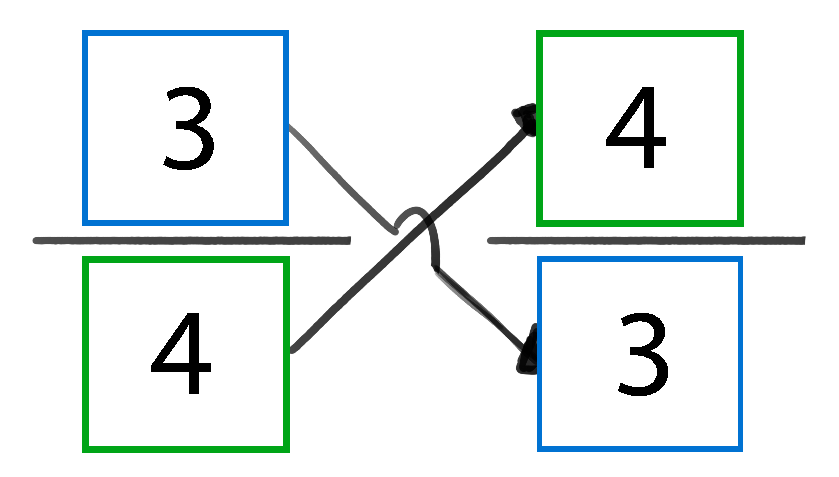
\includegraphics[width=3cm]{img/Inverse002.pdf}
\end{center}

Pour rappel, tout nombre entier peut être écrit sous forme d'une fraction.
\begin{center}
  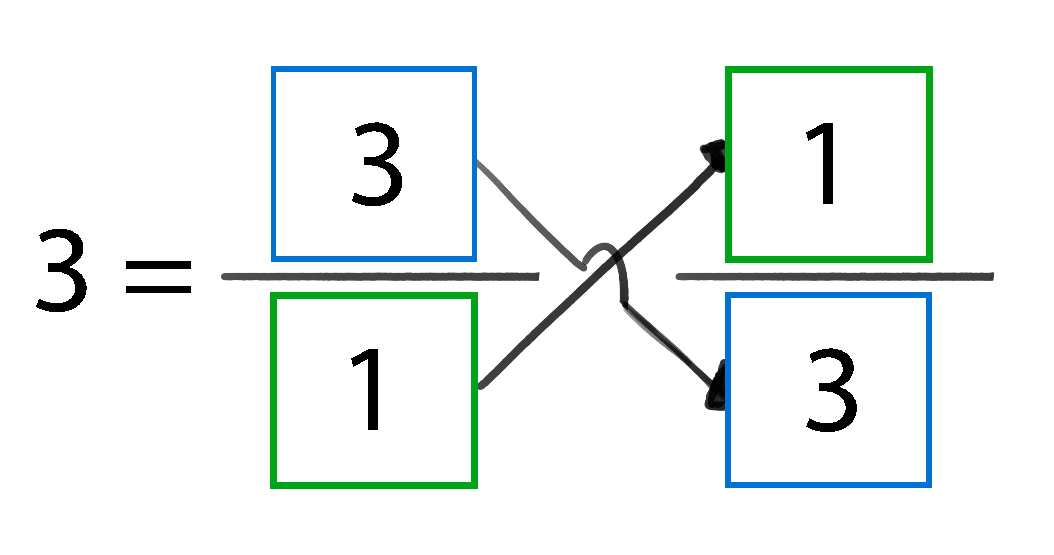
\includegraphics[width=3cm]{img/Inverse003_Entiers.pdf} 
\end{center}

Enfin, il est important de ne pas confondre inverse et opposé d'un nombre.
Pour déterminer l'opposé d'un nombre, il faut changer le signe.\\

\exemples Détermine l'opposé des trois nombres suivants.
\begin{enumerate} [cols=3]
  \item $3 \rightarrow$
  \item $-8 \rightarrow$
  \item $\dfrac{-5}{6} \rightarrow$
\end{enumerate}

\exemples Détermine l'inverse des trois nombres suivants.
\begin{enumerate} [cols=3]
  \item $71 \rightarrow$
  \item $-6 \rightarrow$
  \item $\dfrac{3}{5} \rightarrow$
\end{enumerate}

\begin{exercise}
  Complète les phrases suivantes avec le vocabulaire adéquat.
    \begin{enumerate} [cols=2, itemsep=1cm] 
    \item $\dfrac{5}{9}$ est \dotfill$\dfrac{9}{5}$
    \item $\dfrac{-1}{9}$ est \dotfill$9$
    \item $\dfrac{9}{-5}$ est \dotfill$\dfrac{-9}{5}$
    \item $\dfrac{8}{3}$ est \dotfill$\dfrac{-8}{3}$ 
  \end{enumerate}
\end{exercise}

\begin{exercise}
  Choisis une fraction. Prends son inverse. Multiplie-les ensemble.\\
  Que vaut le produit? Déduis-en une propriété.
\end{exercise}

\newpage

\subsection{Effectuer une division}
Pour diviser une fraction par une autre, il faut~:
\begin{enumerate}[label=\arabic*]
  \item Réduire au maximum les fractions
  \item Multiplier la première fraction par \textbf{l'inverse de la seconde fraction}
\end{enumerate}

\exemple

\begin{enumerate}[cols=2, itemsep=3cm]
  \item $\dfrac{9}{4} : \dfrac{36}{3}=$
  \item $-\dfrac{8}{12} : \dfrac{16}{9}=$
\end{enumerate}

\vspace{3cm}

\begin{exercise}
  Effectue. Veille à ce que ton résultat soit irréductible.
  \begin{enumerate}[cols=2, itemsep=3cm]
    \item $\dfrac{6}{3} : \dfrac{7}{2}=$
    \item $\dfrac{-3}{8} : \dfrac{-27}{-16}=$
    \item $3 : \dfrac{1}{3}=$
    \item $\dfrac{-81}{24} : \dfrac{-18}{4}=$
  \end{enumerate}
\end{exercise}

\newpage

\begin{exercise}
  Effectue. Veille à ce que ton résultat soit irréductible.
  \begin{enumerate}[cols=2, itemsep=3cm]
    \item $\widefrac{\dfrac{3}{2}}{\dfrac{27}{8}}=$
    \item $\widefrac{\dfrac{-50}{9}}{\dfrac{125}{45}}=$
    \item $\widefrac{-\dfrac{2}{9}}{\dfrac{18}{27}}=$
    \item $\widefrac{\dfrac{72}{12}}{2}=$
  \end{enumerate}
\end{exercise}
\vspace{3cm}

\begin{exercise}
  Les $\dfrac{2}{5}$ d'un nombre valent $\dfrac{9}{7}$. Quel est ce nombre?
\end{exercise}

\vspace{4cm}

\begin{exercise}
  Si on multiplie 24 par une fraction, on obtient $\dfrac{9}{8}$. Quelle est cette fraction?
\end{exercise}

\newpage

\section{Priorité des opérations dans les rationnels}
Les fractions étant des nombres, on utilise les mêmes règles de priorité des opérations que dans les entiers.
\\
Pour rappel, cette règle est~:\vspace*{3cm}

\exemple $\dfrac{3}{2} + \dfrac{5}{6} \cdot \dfrac{1}{4}$
\vspace*{4cm}

\begin{exercise}
  (Sur feuille annexe) Effectue. Laisse ta démarche visible.
  \begin{enumerate}[cols=2]
    \item $\dfrac{3}{2}+\left(\dfrac{1}{5}\cdot \dfrac{15}{7}\right)\cdot 7$
    \item $\dfrac{2}{3}-\left(\dfrac{5}{3}-\dfrac{3}{2}\right)\cdot 6$
    \item $\left(\dfrac{3}{4}-\dfrac{1}{2}\right)^2+\dfrac{7}{8}$
    \item $\dfrac{16}{18} : \dfrac{8}{27}+1,1$
    \item $0,7-\dfrac{3}{7} \cdot \dfrac{49}{18}$
    \item $\left(\dfrac{1}{3}\right)^3 + \dfrac{8}{4}$
    \item $3+\dfrac{7}{9}-\dfrac{1500}{-600}$
    \item $\left(\dfrac{3}{36}-\dfrac{7}{4}\right) \cdot \left(\dfrac{15}{35}+\dfrac{-2}{28}\right)$
  \end{enumerate}
\end{exercise}


\begin{exercise}
  (Sur feuille annexe) Sachant que $p=\dfrac{-3}{2}$ et que $m=\dfrac{1}{3}$, calcule la valeur de $w$ dans l'expression suivante.
  \vspace{0.5cm} %Ma vision esthétique
  \[w=3p-p^3+mp+6m\]
\end{exercise}

\newpage
\section{Exercices mélangés}
\setcounter{exercise}{0}
\textbf{Rappel : sauf si l'énoncé dit autre chose, le résultat doit être irréductible.}
\subsection{Exercices de drill}

\begin{exercise}
  Effectue. 
  \begin{enumerate}[cols=3]
    \item $\dfrac{-80}{-90}- \dfrac{-3}{8}$
    \item $\dfrac{3}{-5} +7$
    \item $\dfrac{-6}{18} +\dfrac{6}{15}$    
    \item $\dfrac{3}{5}+\dfrac{7}{5}-5$
    \item $11 + \dfrac{11}{6}- \dfrac{7}{9}$
    \item $\dfrac{-1}{3}- \dfrac{1}{7}$
    \item $\dfrac{8}{2}- \dfrac{3}{4}$
    \item $\dfrac{45}{75}- \dfrac{7}{15}$
    \item $\dfrac{14}{6} + \dfrac{-8}{7}$
    \item $\dfrac{-100}{18}+ \dfrac{25}{9}$
    \item $\dfrac{-3}{7} +\dfrac{5}{7} - \dfrac{29}{14}$
    \item $\dfrac{8}{16}+\dfrac{7}{9}$
    \item $\dfrac{4}{9}+\dfrac{6}{8}$
    \item $\dfrac{5}{12}+\dfrac{12}{-20}$
    \item $\dfrac{18}{15} - \dfrac{28}{27}$
  \end{enumerate}
\end{exercise}

\begin{exercise}
  Effectue.
  \begin{enumerate}[cols=3]
    \item $\dfrac{-45}{18} \cdot \dfrac{27}{-100}$    \item $4,5 \cdot \dfrac{16}{32}$
    \item $\dfrac{7}{8} \cdot \dfrac{42}{49}\cdot\dfrac{12}{14}$
    \item $\dfrac{-100}{-54} \cdot \dfrac{18}{25}$
    \item $\dfrac{64}{48} \cdot \dfrac{6}{56}$
    \item $\dfrac{-24}{-80} \cdot \dfrac{-10}{72}$
    \item $5 \cdot \dfrac{13}{15}$
    \item $\dfrac{50}{100} \cdot \dfrac{1}{4}$
    \item $\dfrac{7}{6} \cdot \dfrac{12}{49}$
  \end{enumerate}
\end{exercise}

\begin{exercise}
  Effectue. 
  \begin{enumerate}[cols=3]
    \item $\dfrac{\dfrac{2}{3}}{\dfrac{18}{8}}$
    \item $\dfrac{-8}{15} : \dfrac{16}{20} $
    \item $\dfrac{-60}{40} : \dfrac{-9}{6} $
    \item $\dfrac{12}{24} : 7,2$
    \item $\dfrac{\dfrac{-18}{42}}{\dfrac{27}{-8}} $
    \item $\dfrac{50}{12} : \dfrac{25}{42} $
    \item $8 : \dfrac{1}{2} $
    \item $\dfrac{-28}{81} : \dfrac{49}{27} $
    \item $\dfrac{-8}{52} : \dfrac{56}{13} $
  \end{enumerate}
\end{exercise}

\newpage
\begin{exercise}
  Effectue. N'oublie pas de simplifier la fraction si possible avant de commencer. 
  \begin{enumerate}[cols=3]
    \item $\left(\dfrac{12}{18}\right)^3$
    \item $\left(\dfrac{-5}{9}\right)^2$
    \item $\left(\dfrac{18}{35}\cdot\dfrac{14}{9}\right)^3$
    \item $\left(\dfrac{-81}{-27}\right)^2$
    \item $\left(\dfrac{4}{14}\right)^2$
    \item $\left(\dfrac{-14}{28}\right)^5$
    \item $\left(-\dfrac{-4}{8}\right)^3$
    \item $\left(\dfrac{12}{-15}\right)^2$
    \item $\left(\dfrac{10}{6} + 1\right)^2$
  \end{enumerate}
\end{exercise}

\begin{exercise}
  Effectue.
  \begin{enumerate}[cols=2]
    \item $\dfrac{1}{3}-2\cdot\dfrac{1}{2}$
    \item $\left(2-\dfrac{1}{4}\right) \cdot \dfrac{1}{3}$
    \item $\dfrac{8}{14} + \dfrac{9}{7}$
    \item $\left(\dfrac{14}{16}\right)^2$
    \item $\left(\dfrac{-90}{72} \cdot \dfrac{16}{-100}\right) + \dfrac{5}{10} $
    \item $\dfrac{6}{24} - \left(\dfrac{7}{2}\right)^2$
    \item $\dfrac{-4}{10} : \dfrac{18}{50} \cdot \dfrac{27}{5}$
    \item $\left(\dfrac{4}{3} + \dfrac{8}{27}\right) - \dfrac{12}{18}$
     \item $\dfrac{-8}{7} : \dfrac{21}{-2}$
    \item $\dfrac{40}{25} : \dfrac{8}{75}$
    \item $1,5\cdot \dfrac{18}{12}$
    \item $\dfrac{5}{15} + 3$
    \item $\dfrac{11}{6} - \dfrac{-7}{9}$
    \item $8 \cdot \dfrac{15}{10}$
    \item $\left(\dfrac{3}{8}\right)^2$

  \end{enumerate}
\end{exercise}

\newpage
\subsection{À toi de jouer}
\begin{exercise}
  Effectue. Laisse ta démarche visible et veille à ce que ton résultat soit le plus simplifié possible.
  \begin{enumerate}[cols=2]
    \item $\left(\dfrac{1}{2}+\dfrac{-1}{3}\right) \cdot \left(\dfrac{1}{4}+\dfrac{1}{-5}\right)$
    \item $\dfrac{-3}{8}\cdot \left(\dfrac{12}{9}\right)^2$
    \item $-\dfrac{7}{2}+\dfrac{-9}{45} - \dfrac{22}{15}$
    \item $3+\dfrac{5}{7} - \dfrac{-5}{8}$
    \item $\dfrac{4}{45}-\left(\dfrac{-75}{25} - \dfrac{8}{15}\right)$
    %\item $\dfrac{3}{2} -4 +\dfrac{8}{7}=$
    \item $\dfrac{45}{15}-\dfrac{7}{30} - \dfrac{4}{21}\cdot \dfrac{28}{16}$
    \item $\left(\dfrac{1}{2}\right)^3 - \dfrac{6}{8} - \dfrac{3}{7} \cdot \dfrac{21}{14}$
  \end{enumerate}
\end{exercise}


\begin{exercise}
  Quelle doit être la valeur de \(a\) dans les fractions ci-dessous~?
  \begin{enumerate}[cols=2]
    \item $\dfrac{a+2}{4}=1$
    \item $\dfrac{4+a}{-5}=1$
    \item $0=\dfrac{3+a}{-1}$
    \item $\dfrac{28}{20-a}=2$
  \end{enumerate}
\end{exercise}

\begin{exercise}
  Écris la fraction $\dfrac{16}{9}$ sous la forme \dots\\
  \begin{enumerate}
    \item \dots d'un produit de deux fractions égales.
    \item \dots d'un produit de deux fractions différentes.
    \item \dots d'un quotient de deux fractions.
    \item \dots d'une somme de deux fractions égales.
  \end{enumerate}
\end{exercise}

\begin{exercise}
  En simplifiant la fraction $\dfrac{a}{b}$, on obtient $\dfrac{1}{8}$. Leur PGCD vaut 15. Quelle est la fraction de départ?
\end{exercise}

\begin{exercise}
  Théo remarque qu'il a déjà utilisé \(\dfrac{4}{5}\) de son forfait GSM ce mois-ci. Il utilise les \(\dfrac{5}{6}\) de ce qu'il lui reste pour appeler Lina. De quelle fraction de son forfait dispose-t-il encore~? \\
  Laisse ta démarche visible.
\end{exercise}

\newpage
\begin{exercise}
  La mère de Gabriel utilise le tiers de son salaire pour le loyer de l'appartement, le huitième pour l'alimentaire, et le quart de ce qu'il reste pour les activités parascolaires de ses enfants. 
  \begin{tasks}
    \task Quelle fraction de son salaire lui reste-t-il pour les loisirs~?
    \task Si elle gagne 1800€ par mois, combien cela représente-t-il~?
  \end{tasks}
\end{exercise}

\begin{exercise}
  On prépare une boisson en mélangeant un liquide chocolaté et du lait. \\
  La recette $A$ mélange 3 parts de liquide chocolaté à 2 parts de lait. \\
  La recette $B$ mélange 2 parts de liquide chocolaté à 1 part de lait. \\
  Quel est le mélange qui a le plus le goût du chocolat? Justifie.

  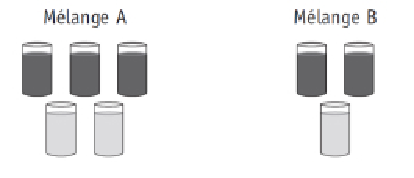
\includegraphics[center]{img/Ex_CE1D.pdf}
  
\end{exercise}

\begin{exercise}
  Calcule la valeur numérique de l'expression $x^3+3x+10$ si $x=\dfrac{-3}{2}$.
\end{exercise}

\begin{exercise}
  Rania veut planter des fleurs sur un quart de son jardin, et créer une marre sur les trois dixièmes de son jardin. Sur la surface qu'il lui reste, elle compte semer de l'herbe. \\
  Quelle proportion de son jardin sera semé d'herbe?  \\ Laisse ta démarche visible.
\end{exercise}

\begin{exercise}
  Calcule l'aire et le périmètre de la figure ci-contre. \\
  Veille à ce que ton résultat soit irréductible.
\begin{center}
  \begin{tikzpicture}
    \tkzDefPoint(0,0){A}
    \tkzDefPoint(0,-4){B}
    \tkzDefPoint(2,-4){C}
    \tkzDefPoint(2,0){D}
    \tkzDrawPolygon(A,B,C,D)
    \tkzLabelPoints[above left](A)
    \tkzLabelPoints[above right](D)
    \tkzLabelPoints[below right](C)
    \tkzLabelPoints[below left](B)
    \tkzLabelSegment(A,D){$\dfrac{2}{7}$} 
    \tkzLabelSegment[right](C,D){$\dfrac{1}{3}$} 
    \tkzDrawPoints(A,B,C,D)
\end{tikzpicture}
\end{center}
\end{exercise}

\begin{exercise}
  Un Belge sur trois est wallon. Si deux Wallons sur cinq sont fumeurs, quelle est la proportion des Wallons fumeurs dans la population belge? 
\end{exercise}

\begin{exercise}
  Daniel a mangé une tablette de \SI{200}{g} de chocolats. L'emballage indique \og 55 \% de sucre \fg. Quelle quantité de sucre a-t-il ingurgitée ?
\end{exercise}

\end{document}